\documentclass[11pt]{article}
\usepackage[margin=1in]{geometry}
\usepackage{graphicx}
\usepackage{booktabs}
\usepackage{hyperref}
\usepackage{longtable}
\usepackage{array}
\usepackage{xcolor}
\usepackage{listings}

\hypersetup{
  colorlinks=true,
  linkcolor=blue!50!black,
  urlcolor=blue!50!black
}

\lstset{
  basicstyle=\ttfamily\small,
  breaklines=true,
  frame=single,
  framerule=0.2pt
}

\title{newspaper-parsing: End-to-End Pipeline Walkthrough}
\author{Saul Richardson + Codex}
\date{February 13, 2026}

\begin{document}
\maketitle

\section{Goal}
This repository formalizes a single production pipeline for newspaper parsing:
\begin{itemize}
  \item Paddle layout detectors: \texttt{PP-DocLayoutV2}, \texttt{PP-DocLayoutV3}, \texttt{PP-DocLayout\_plus-L}
  \item Paddle VL parser: \texttt{doc\_parser v1.5}
  \item Dell layout parser
  \item MinerU2.5 layout parser
  \item Fusion with anti-noise gating
  \item Fused-region transcription with Paddle OCR
\end{itemize}

\section{Pipeline Stages}
\begin{enumerate}
  \item \texttt{paddle\_layout}
  \item \texttt{paddle\_vl15}
  \item \texttt{dell}
  \item \texttt{mineru}
  \item \texttt{fusion}
  \item \texttt{review}
  \item \texttt{transcription}
\end{enumerate}

\noindent
Transcription is ROI-first: Paddle OCR runs on a cleaned non-redundant subset of fused
\texttt{text/title} boxes, then OCR lines are remapped to page coordinates and serialized in fused reading order.

Run all stages:
\begin{lstlisting}
newsbag run --config configs/pipeline.torch.json \
  --stages paddle_layout,paddle_vl15,dell,mineru,fusion,review,transcription
\end{lstlisting}

\section{Torch Execution Pattern}
Recommended orchestration on Torch is a three-job chain:
\begin{enumerate}
  \item GPU inference (\texttt{l40s\_public} or split-L40S/H200): layout sources only
  \item CPU post-processing (\texttt{cs}): fusion and review bundles
  \item GPU transcription (\texttt{l40s\_public}): Paddle OCR over fused regions
\end{enumerate}

This structure avoids low-GPU-utilization cancellation by keeping CPU-only steps off GPU partitions.

\section{Case Study: 2-Page Mini Run (Corrected Dell)}
\textbf{Run ID:} \texttt{layout\_bagging\_20260213\_024626}\\
\textbf{Pages:}
\begin{itemize}
  \item \texttt{abilene-reporter-news-apr-29-1946-p-19}
  \item \texttt{bakersfield-californian-aug-31-1937-p-14}
\end{itemize}

\textbf{Source root (Torch):}
\texttt{/scratch/\$USER/paddleocr\_vl15/runs/layout\_bagging\_20260213\_024626}

\subsection{Visual Outputs}
\begin{figure}[h]
\centering
\includegraphics[width=0.92\textwidth]{images/mini_run/abilene_input.png}
\caption{Mini run input page (Abilene).}
\end{figure}

\begin{figure}[h]
\centering
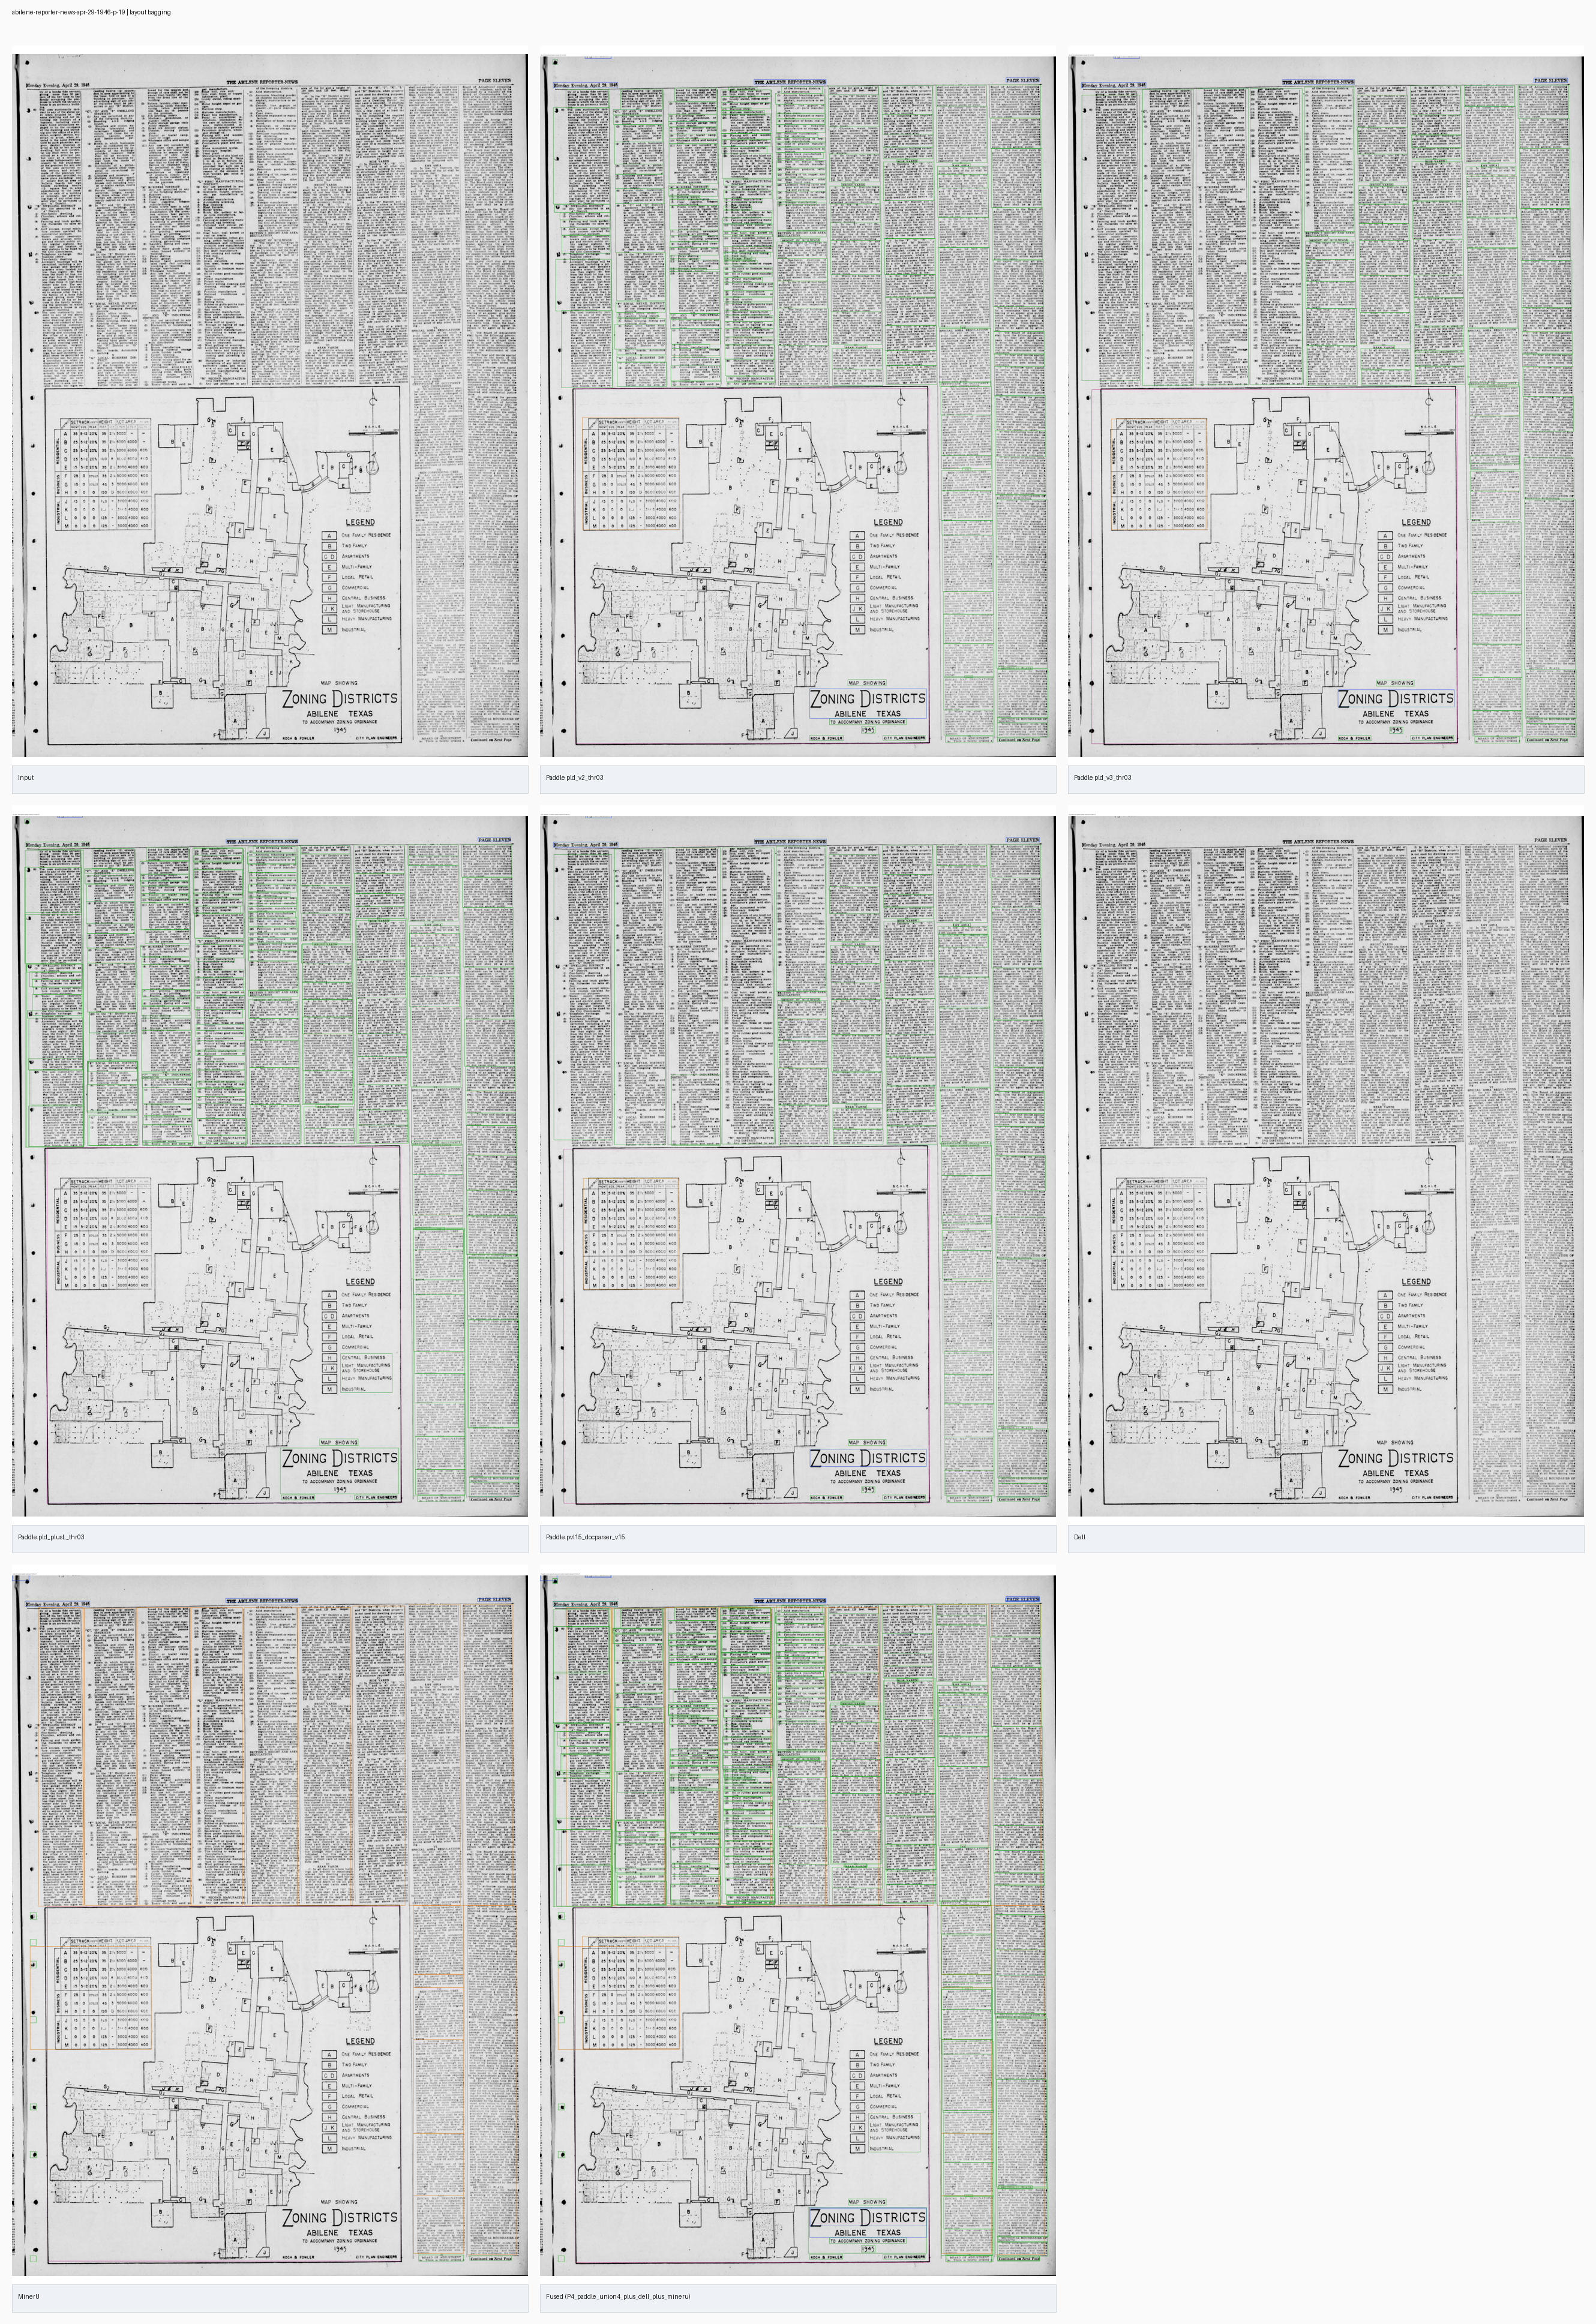
\includegraphics[width=0.92\textwidth]{images/mini_run/abilene_board.png}
\caption{Abilene full model board: Paddle4, Dell, MinerU, fused result.}
\end{figure}

\begin{figure}[h]
\centering
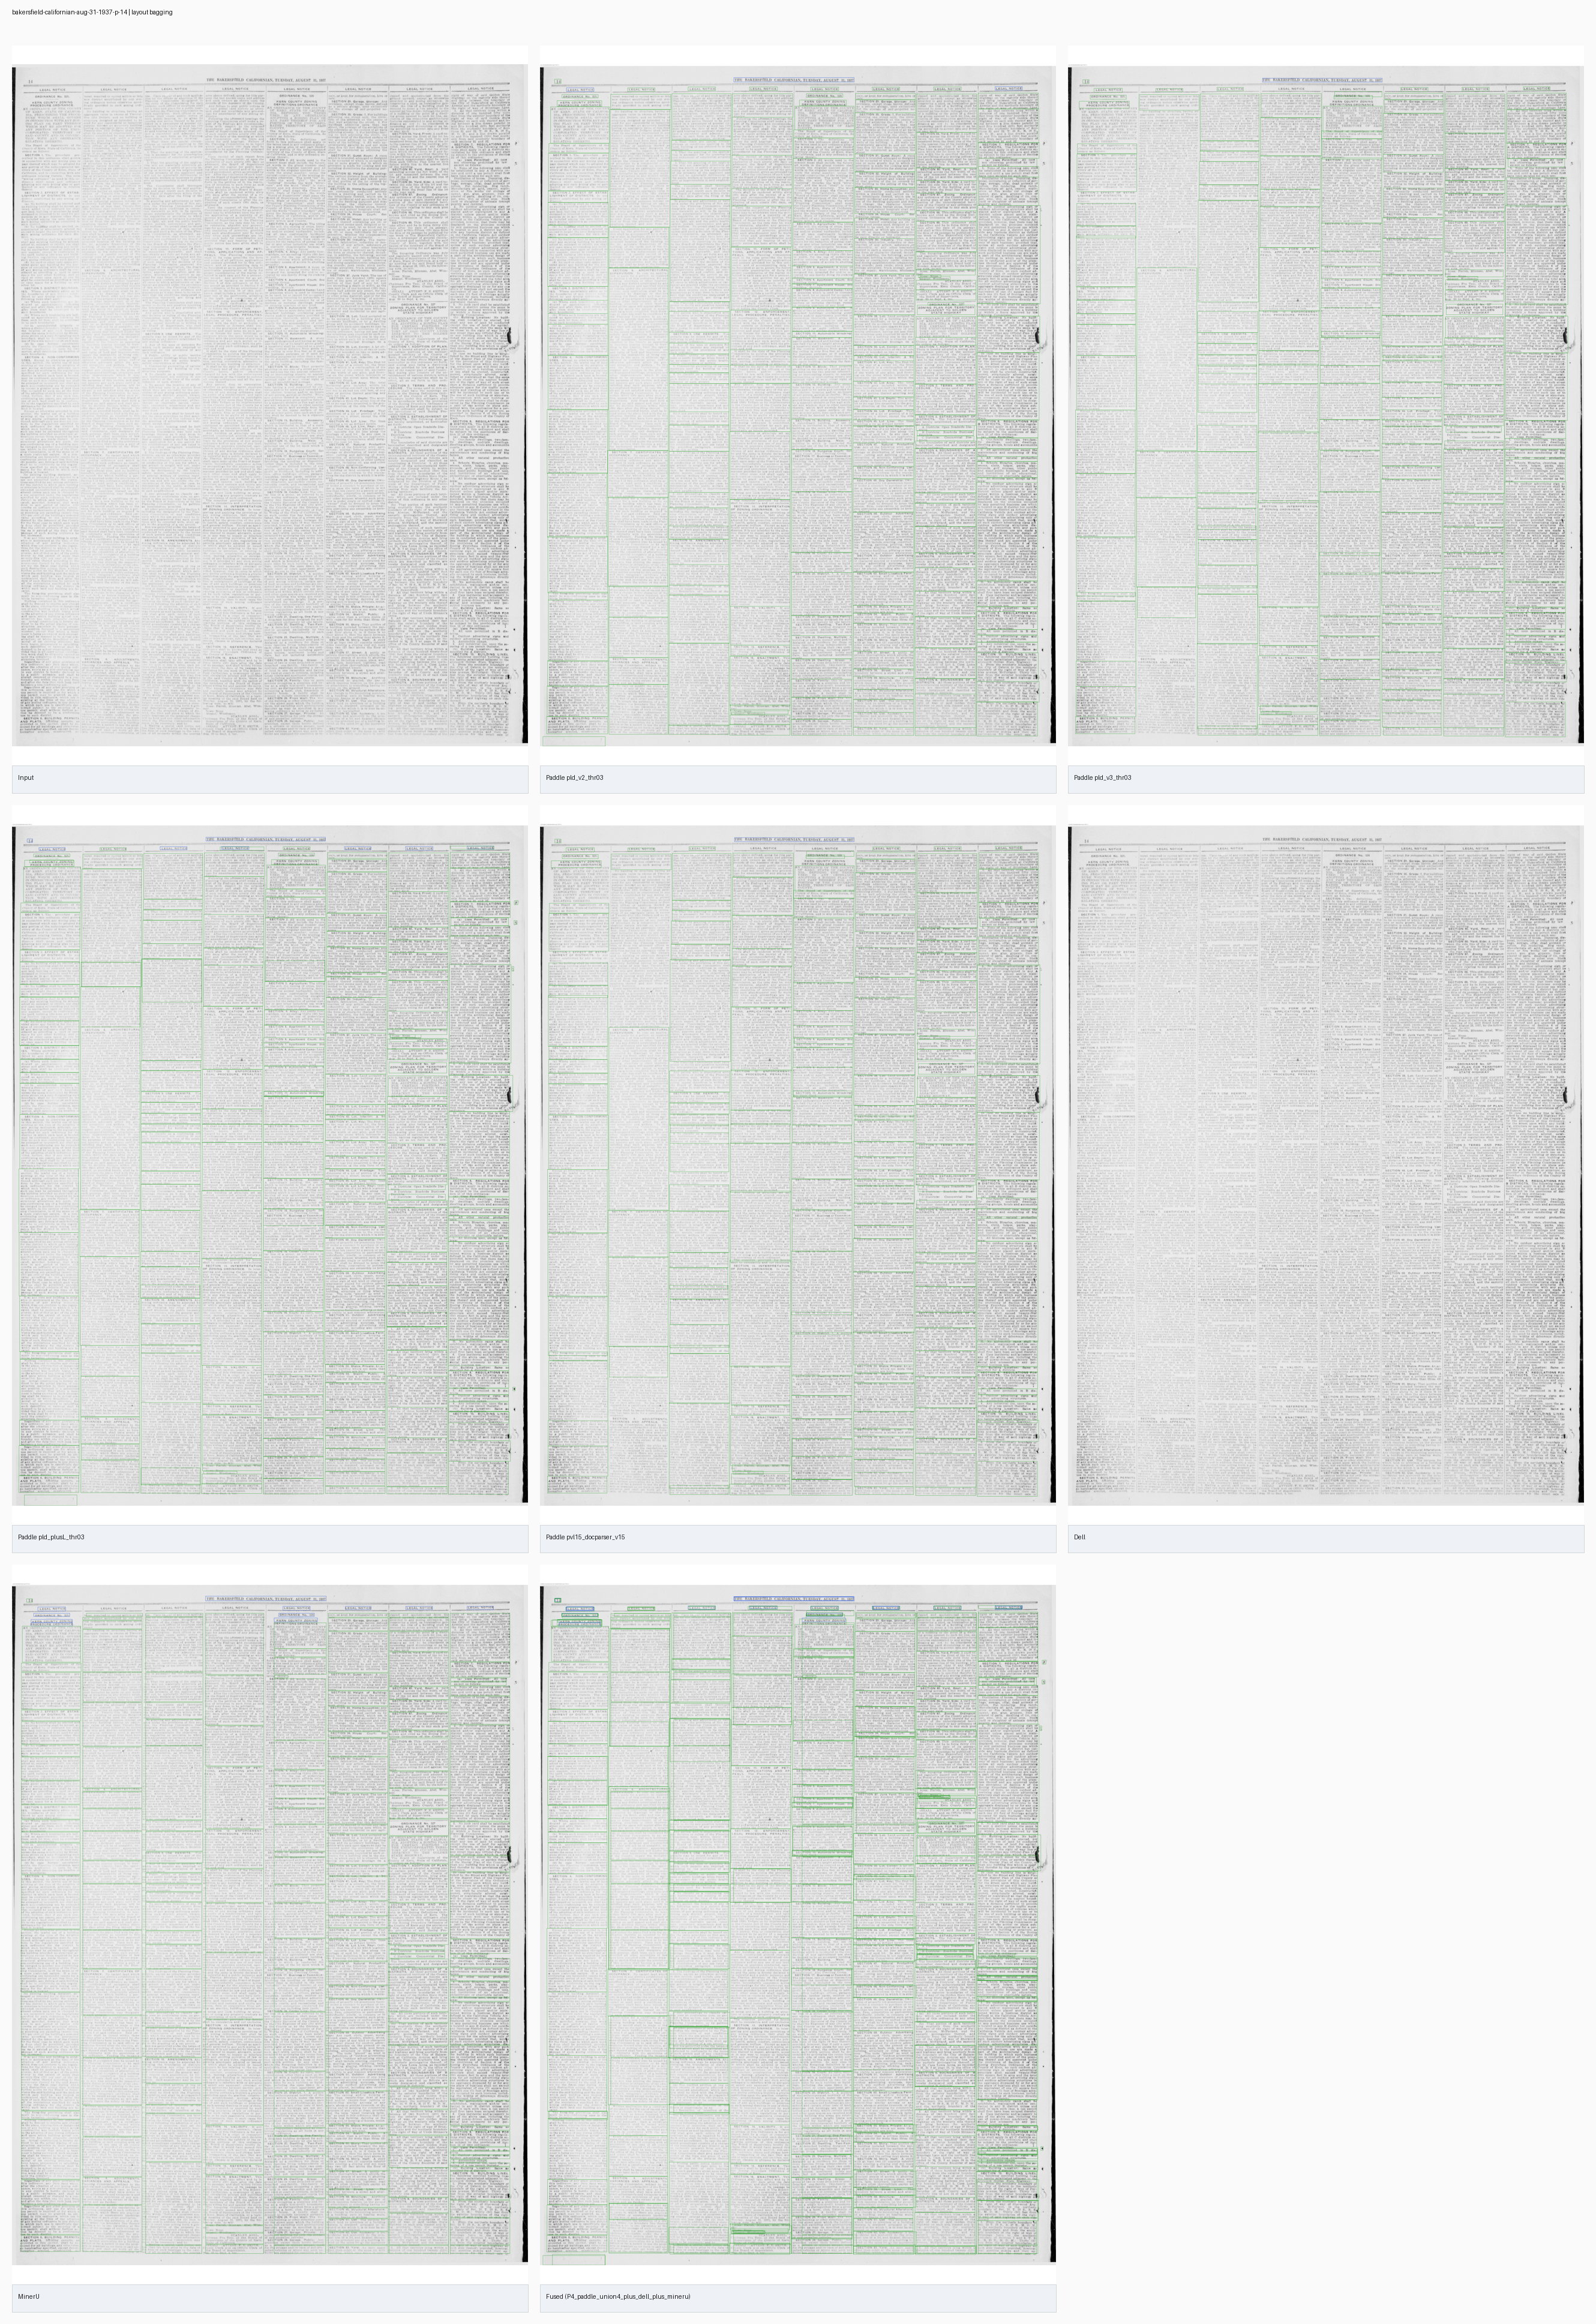
\includegraphics[width=0.92\textwidth]{images/mini_run/bakersfield_board.png}
\caption{Bakersfield full model board: Paddle4, Dell, MinerU, fused result.}
\end{figure}

\begin{figure}[h]
\centering
\includegraphics[width=0.92\textwidth]{images/mini_run/bakersfield_miner_delta.png}
\caption{Bakersfield with/without MinerU panel (\texttt{P2} vs \texttt{P4}).}
\end{figure}

\begin{figure}[h]
\centering
\includegraphics[width=0.92\textwidth]{images/mini_run/abilene_dell_layout.png}
\caption{Abilene Dell-only overlay after runner fix (non-empty output).}
\end{figure}

\clearpage
\subsection{Actual Metrics (from Run Artifacts)}
Variant leaderboard excerpt (\texttt{outputs/fusion/variant\_leaderboard.tsv}):
\begin{center}
\begin{tabular}{lrrr}
\toprule
Variant & Mean Base Recall & Mean Text Area & Mean Boxes \\
\midrule
\texttt{P2\_paddle\_union4\_plus\_dell} & 0.997774 & 0.737427 & 329.0 \\
\texttt{S1\_paddle\_best\_single} & 0.966463 & 0.698220 & 224.5 \\
\texttt{P4\_paddle\_union4\_plus\_dell\_plus\_mineru} & 0.997929 & 0.738797 & 404.5 \\
\bottomrule
\end{tabular}
\end{center}

Source leaderboard excerpt (\texttt{outputs/fusion/source\_leaderboard.tsv}):
\begin{center}
\begin{tabular}{lrrr}
\toprule
Source & Mean Base Recall & Mean Text Area & Mean Boxes \\
\midrule
\texttt{pld\_plusL\_thr03} & 0.979841 & 0.698220 & 224.5 \\
\texttt{pld\_v2\_thr03} & 0.958174 & 0.689416 & 209.5 \\
\texttt{dell\_c0005\_i010} & 0.884912 & 0.584741 & 25.0 \\
\texttt{mineru25} & 0.473897 & 0.427513 & 125.0 \\
\bottomrule
\end{tabular}
\end{center}

\subsection{Dell Output Verification}
The corrected Dell runner produced non-empty outputs on both pages:
\begin{itemize}
  \item \texttt{abilene-reporter-news-apr-29-1946-p-19}: 23 boxes
  \item \texttt{bakersfield-californian-aug-31-1937-p-14}: 28 boxes
\end{itemize}
Counts are from:
\texttt{outputs/sources/dell/dell\_c0005\_i010/<slug>/layout\_boxes.normalized.json}

\subsection{Transcription Outputs}
Generated artifacts:
\begin{itemize}
  \item \texttt{outputs/transcription/P4\_paddle\_union4\_plus\_dell\_plus\_mineru/transcription\_report.tsv}
  \item \texttt{outputs/transcription/P4\_paddle\_union4\_plus\_dell\_plus\_mineru/transcript\_combined.txt}
  \item Per-page:
    \begin{itemize}
      \item \texttt{ocr\_raw.json}
      \item \texttt{ocr\_lines.json}
      \item \texttt{transcript\_boxes.json}
      \item \texttt{transcript.txt}
      \item \texttt{ocr\_regions\_overlay.png}
      \item \texttt{ocr\_lines\_overlay.png}
    \end{itemize}
\end{itemize}

\textbf{Transcription report excerpt:}
\begin{center}
\begin{tabular}{lrrrrr}
\toprule
Slug & Fused Boxes & OCR Regions & OCR Lines & Assigned Lines & Transcript Chars \\
\midrule
\texttt{abilene...p-19} & 331 & 54 & 3814 & 3814 & 32396 \\
\texttt{bakersfield...p-14} & 457 & 112 & 2871 & 2871 & 31760 \\
\bottomrule
\end{tabular}
\end{center}

\textbf{OCR region reduction in this run:}
\begin{itemize}
  \item \texttt{abilene...p-19}: 331 fused boxes $\rightarrow$ 54 OCR regions
  \item \texttt{bakersfield...p-14}: 457 fused boxes $\rightarrow$ 112 OCR regions
\end{itemize}

\begin{figure}[h]
\centering
\includegraphics[width=0.92\textwidth]{images/mini_run/abilene_ocr_regions_overlay.png}
\caption{Abilene OCR regions actually passed to Paddle OCR after overlap cleaning.}
\end{figure}

\begin{figure}[h]
\centering
\includegraphics[width=0.92\textwidth]{images/mini_run/abilene_ocr_lines_overlay.png}
\caption{Abilene remapped OCR line boxes on the original page.}
\end{figure}

\section{What to Inspect First}
\begin{enumerate}
  \item \texttt{review/pages/<slug>/06\_board.png}
  \item \texttt{review/pages/<slug>/07\_with\_vs\_without\_miner.png}
  \item \texttt{outputs/fusion/variant\_leaderboard.tsv}
  \item \texttt{outputs/transcription/<variant>/transcription\_report.tsv}
  \item \texttt{outputs/transcription/<variant>/<slug>/transcript.txt}
\end{enumerate}

\section{Reproducibility Notes}
\begin{itemize}
  \item The run writes \texttt{manifests/config.resolved.json} and \texttt{manifests/images.resolved.txt}.
  \item Torch config is pinned to a compute-node-valid Paddle binary:
  \texttt{/scratch/\$USER/paddleocr\_vl15/venv\_gpu\_l40s\_py39/bin/paddleocr}
  \item Slurm wrappers now re-install editable package automatically if the active \texttt{newsbag} import path drifts outside \texttt{PROJECT\_ROOT}.
  \item External-source fail-fast checks are now first-class:
  \texttt{dell.min\_nonempty\_pages} and \texttt{mineru.min\_nonempty\_pages}.
  If a source is empty across all processed pages, the run exits before fusion/review.
\end{itemize}

\end{document}
